\documentclass{beamer}
\usepackage[utf8]{inputenc}
\usepackage{graphicx}
\usepackage{amsmath}
\usepackage{booktabs}
\usepackage{textcomp}
\usepackage{multirow}
\usepackage{color}
\usepackage[ngerman]{babel}
\usetheme{Dresden}
\title{Moose FS}
\author{Ralph Krimmel}

\begin{document}

\section{Einleitung}
\subsection*{}
\begin{frame}
	\maketitle
\end{frame}


%\begin{frame}{Definition}
%In computing, a distributed file system or network file system is any file system that allows access to files from multiple hosts via a computer network.$[1]$
%\tiny{$[1]$ Galvin Silberschatz (1994). Operating System concepts, chapter 17 Distributed file systems. Addison-Wesley Publishing Company.} \\
%\end{frame}

%\begin{frame}{Nichts neues...}

%z.B. NFS, entwickelt von Sun Microsystems in 1984
%\begin{itemize}
%\item Schlechte Performanz bei vielen Clients \\ $\Rightarrow$ Skaliert nicht
%\item Keine Fehlertoleranz
%\end{itemize}
%\end{frame}

%\begin{frame}{Anforderungen an ein modernes, verteiltes Dateisystem}
%	\begin{itemize}
%	\item Hohe Performanz durch Striping
%	\begin{itemize}
%		\item Durchsatz
%		\item Latenz
%	\end{itemize}
%	\item Skalierbarkeit
%	\item Verf\"ugbarkeit
%	\item Zuverl\"assigkeit
%	\end{itemize}
%\end{frame}

%\begin{frame}{Zuverl\"assigkeit/Verf\"ugbarkeit}
%	Problem: Fehler sind mehr die Norm als die Ausnahme
%\begin{itemize}
%	\item System g\"unstiger Hardware
%	\item Fehler in Programmen %theres software that always crashes
%	\item Menschliches Versagen % what was this cable for?
%	\item Betriebssystemfehler % ever used windows?
%	\item Ausfall von:
%	\begin{itemize}
%		\item Festplatten
%		\item Arbeitsspeicher
%		\item Netzwerk
%		\item ...
%	\end{itemize}
%\end{itemize}	
%\end{frame}

%\begin{frame}{Moderner Ansatz}
%	\begin{itemize}
%	\item Objektbasiert $\rightarrow$ Object storage devices (OSD's)
%	\begin{itemize}
%		\item CPU
%		\item Festplatten 
%		\item Netzwerkschnittstelle
%		\item Lokaler Cache
%	\end{itemize}
%	\item Metadaten getrennt von Nutzdaten
%	\end{itemize}
%\end{frame}

\begin{frame}
	\frametitle{Verteilte Dateisysteme}
	\begin{columns}
	\column{.55\textwidth}
	\begin{block}{Viele bekannte Namen}
	\begin{itemize}
		\item Ceph
		\item Lustre
		\item Glusterfs
		\item ...
	\end{itemize}
	\end{block}
	\column{.45\textwidth}
	
\includegraphics[scale=0.22]{ceph.jpg}

	\vspace{0.8cm}	
	
\includegraphics[scale=0.2]{lustre.png}
	
	
\includegraphics[scale=0.2]{gluster.jpg}
	\end{columns}
\end{frame}

\begin{frame}
	\frametitle{Eher unbekannt: Moose FS}
	\centering
	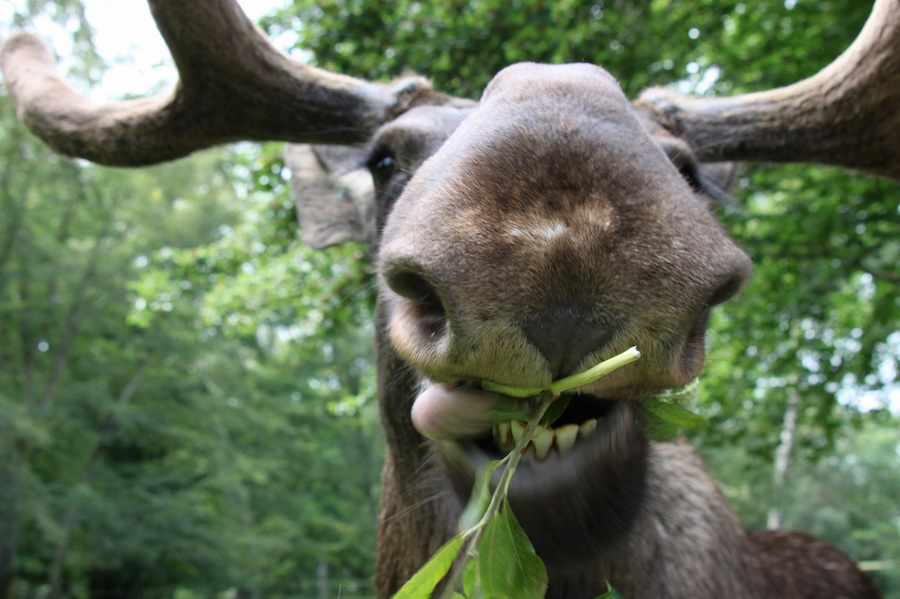
\includegraphics[scale=0.3]{elch1.jpg}
\end{frame}

\begin{frame}
	\frametitle{Eher unbekannt: Moosefs}
	\begin{columns}	
	\column{.45\textwidth}
	
\includegraphics[scale=0.5]{moosefs.jpg}
	\column{.55\textwidth}
	\begin{block}{Standard Features}
		\begin{itemize}
			\item Hierarchisch (Baumstruktur)
			\item POSIX Datei Attribute:
			\begin{itemize}
				\item POSIX Rechte
				\item Last Access Time
				\item Modification Time 
			\end{itemize}	
			\item Spezialdateien
			\begin{itemize}
				\item Pipes
				\item Sockets
				\item Blockdevices
			\end{itemize}
			\item Symbolische und Hardlinks
		\end{itemize}
	\end{block}	
	\end{columns}
\end{frame}

\begin{frame}
	\frametitle{Eher unbekannt: Moosefs}
	\begin{columns}	
	\column{.45\textwidth}
	
\includegraphics[scale=0.5]{moosefs.jpg}
	\column{.55\textwidth}
	\begin{block}{weitere, besondere Features:}
		\begin{itemize}
			\item Einstellbar hohe Zuverlaessigkeit
			\item Einfach skalierbar
			\item \glqq M\"ulleimer\grqq -funktion
			\item Koh\"arente Snapshots
		\end{itemize}
	\end{block}	
	\end{columns}
\end{frame}



\section{MFS Technik}
\subsection*{}
		
\begin{frame}
	\frametitle{MFS Architektur}
	\begin{block}{4 Komponenten}
	\begin{itemize}
		\item Master server
		\item Chunk server
		\item Metalogger server
		\item MFS Client: mfsmount
	\end{itemize}
	\end{block}
\end{frame}

\begin{frame}
	\frametitle{Master und Chunkserver}
	\begin{block}{mfsmaster}
	\begin{itemize}
		\item Verwaltung von Metadaten
		\item Verwaltung/Weiterleitung von Lese/Schreizugriffen
	\end{itemize}
	\end{block}

	\begin{block}{mfschunkserver}
	\begin{itemize}	
		\item Objektspeicher
		\item Eigenst\"andiges Vervielf\"altigen 
	\end{itemize}
	\end{block}
\end{frame}

\begin{frame}
	\frametitle{Metalogger und Client}

	\begin{block}{mfsmetalogger}
	\begin{itemize}
		\item Regelm\"assiges kopieren der Metadaten vom Master
	\end{itemize}
	\end{block}

	\begin{block}{mfsmount}
	\begin{itemize}
		\item Zugriff auf das Moose Dateisystem
	\end{itemize}
	\end{block}
\end{frame}

\begin{frame}
	\frametitle{Plattformen}
	\begin{block}{Clients (aka mfsmount): Alle mit funktionierender FUSE Implementierung}
	\begin{itemize}
		\item Linux (ab Version 2.6.14)
		\item FreeBSD
		\item OpenSolaris
		\item MacOS X
	\end{itemize}
	\end{block}
	\begin{block}{Nur Server, Metalogger und Chunkserver}
	\begin{itemize}
		\item Solaris 
		\item Windows mit Cygwin
	\end{itemize}
	\end{block}
\end{frame}


\begin{frame}
	\frametitle{Lesen}
	\centering
	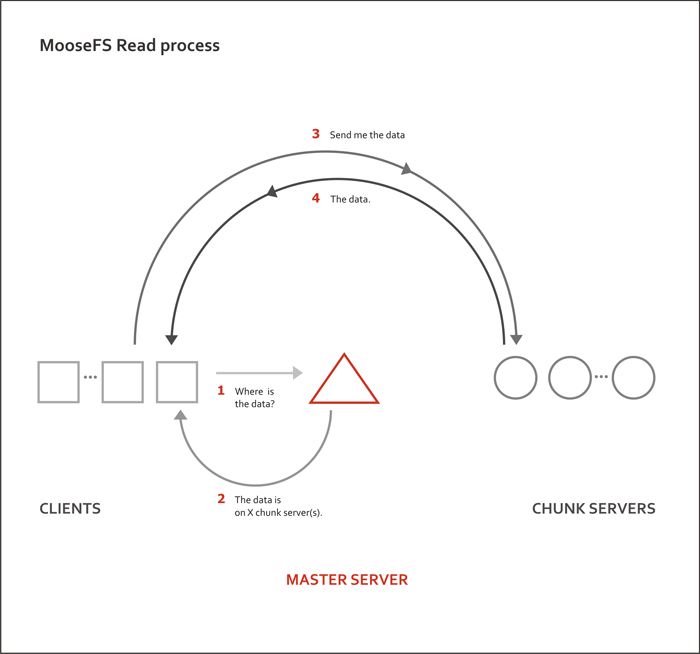
\includegraphics[scale=0.3]{read.png}
\end{frame}

\begin{frame}
	\frametitle{Schreiben}
	\centering
	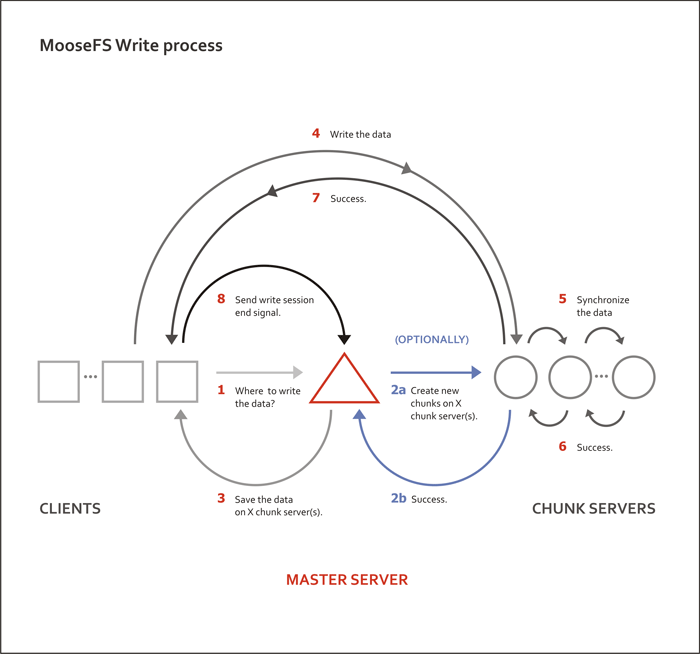
\includegraphics[scale=0.3]{write.png}
\end{frame}


\section{Elchtest}
\subsection*{}

\begin{frame}
	\frametitle{Elchtest - Oder: Wir bauen uns ein guenstiges Netzlaufwerk}
	\centering
	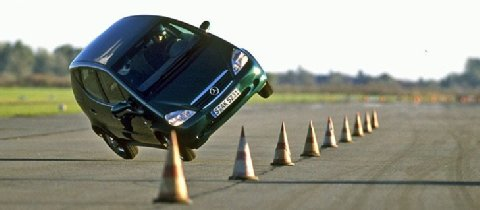
\includegraphics[scale=0.5]{elchtest.jpg}	
\end{frame}

\begin{frame}
	\frametitle{Master}
	\begin{itemize}
	\item	Erreichbar unter \textbf{mooseking.gwdg.de}	
	\item 	Port 9419 f\"ur Metalogger Verbindungen
	\item	Port 9420 f\"ur Chunkserver Verbindungen
	\item	Port 9421 f\"ur Client Verbindungen
	\end{itemize}
\end{frame}
	

\begin{frame}
	\frametitle{Mfscgiserv}
\end{frame}

\begin{frame}
	\frametitle{Beispiel Installation Client: Ubuntu (bis 13.10)}
	\begin{itemize}
		\item apt-add-repository ppa:rquillo/moosefs
		\item apt-get update
		\item apt-get install mfs-client
		\item mkdir /mnt/mfs 
		\item cp /etc/mfs/mfsmount.cfg.dist /etc/mfs/mfsmount.cfg
		\item Konfigurieren des Mountpunktes in /etc/mfs/mfsmount.cfg
		\begin{description}
			\item mfsmaster=mooseking.gwdg.de
			\item /mnt/mfs
		\end{description}
		\item mfsmount
	\end{itemize}
\end{frame}

\section{Fazit}
\subsection*{}

\section{Fragen?}
\subsection*{}

\begin{frame}
	\frametitle{Fragen?}
	\begin{center}
		\large Fragen?
	\end{center}
\end{frame}

\end{document}
